\begin{table}[t]
	\centering
	\begin{tabular}{ccccc}
		\toprule
          & (\ref{tab.h1abcd}a)& (\ref{tab.h1abcd}b)&(\ref{tab.h1abcd}c)&(\ref{tab.h1abcd}d)
\\
	\midrule
New Label	& 
		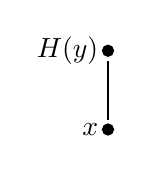
\begin{tikzpicture}[baseline=(current bounding box.center)]
			\node (x) at (0,0) {};
			\node (y) at (0,1) {};
			
			\draw[fill=black] (x) circle (2pt);
			\draw[fill=black] (y) circle (2pt);
			
			\draw (x) -- (y);
			\node[left] at (y) {$H(y)$};
			\node[left] at (x) {$x$};
		\end{tikzpicture}
		&
		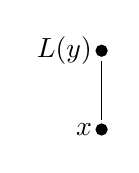
\begin{tikzpicture}[baseline=(current bounding box.center)]
			\node (x) at (0,0) {};
			\node (y) at (0,1) {};
			
			\draw[fill=black] (x) circle (2pt);
			\draw[fill=black] (y) circle (2pt);
			
			\draw (x) -- (y);
			\node[left] at (y) {$L(y)$};;
			\node[left] at (x) {$x$};
		\end{tikzpicture}
		&
		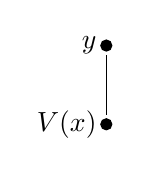
\begin{tikzpicture}[baseline=(current bounding box.center)]
			\node (x) at (0,0) {};
			\node (y) at (0,1) {};
			
			\draw[fill=black] (x) circle (2pt);
			\draw[fill=black] (y) circle (2pt);
			
			\draw (x) -- (y);
			\node[left] at (y) {$y$};
			\node[left] at (x) {$V(x)$};
		\end{tikzpicture}
		&
		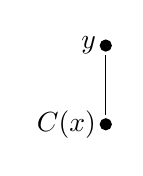
\begin{tikzpicture}[baseline=(current bounding box.center)]
			\node (x) at (0,0) {};
			\node (y) at (0,1) {};
			
			\draw[fill=black] (x) circle (2pt);
			\draw[fill=black] (y) circle (2pt);
			
			\draw (x) -- (y);
			\node[left] at (y) {$y$};
			\node[left] at (x) {$C(x)$};
		\end{tikzpicture}
          \\
          \midrule
&(\ref{tab.h1abcd}e)&(\ref{tab.h1abcd}f)                                                    &(\ref{tab.h1abcd}g)&(\ref{tab.h1abcd}h)\\
          \midrule
New Node	&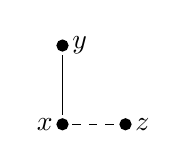
\begin{tikzpicture}[baseline=(current bounding box.center)]
			\node (x) at (0,0) {};
			\node (y) at (0,1) {};
			\node (z) at (0.8,0) {};
			
			\draw[fill=black] (x) circle (2pt);
			\draw[fill=black] (y) circle (2pt);
			\draw[fill=black] (z) circle (2pt);
			
			\draw (x) -- (y);
			\draw[dashed] (x) -- (z);
			
			\node[left] at (x) {$x$};
			\node[right] at (y) {$y$};
			\node[right] at (z) {$z$};
		\end{tikzpicture}
		&
			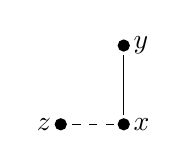
\begin{tikzpicture}[baseline=(current bounding box.center)]
			\node (x) at (0,0) {};
			\node (y) at (0,1) {};
			\node (z) at (-0.8,0) {};
			
			\draw[fill=black] (x) circle (2pt);
			\draw[fill=black] (y) circle (2pt);
			\draw[fill=black] (z) circle (2pt);
			
			\draw (x) -- (y);
			\draw[dashed] (x) -- (z);
			
			\node[right] at (x) {$x$};
			\node[right] at (y) {$y$};
			\node[left] at (z) {$z$};
		\end{tikzpicture}
		&
	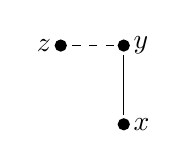
\begin{tikzpicture}[baseline=(current bounding box.center)]
		\node (x) at (0,0) {};
		\node (y) at (0,1) {};
		\node (z) at (-.8,1) {};
		
		\draw[fill=black] (x) circle (2pt);
		\draw[fill=black] (y) circle (2pt);
		\draw[fill=black] (z) circle (2pt);
		
		\draw (x) -- (y);
		\draw[dashed] (y) -- (z);
		
		\node[right] at (x) {$x$};
		\node[right] at (y) {$y$};
		\node[left] at (z) {$z$};
	\end{tikzpicture}
		&
		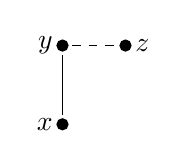
\begin{tikzpicture}[baseline=(current bounding box.center)]
			\node (x) at (0,0) {};
			\node (y) at (0,1) {};
			\node (z) at (.8,1) {};
			
			\draw[fill=black] (x) circle (2pt);
			\draw[fill=black] (y) circle (2pt);
			\draw[fill=black] (z) circle (2pt);
			
			\draw (x) -- (y);
			\draw[dashed] (y) -- (z);
			
			\node[left] at (x) {$x$};
			\node[left] at (y) {$y$};
			\node[right] at (z) {$z$};
		\end{tikzpicture}

           
		\\
		% \midrule
		
		% $\forall g\in D^+, h\in g?$
		% & $\times$ & $\times$ & $\checkmark$ & $\times$
		% \\
		
		% $\forall g\in D^-, h\not\in g?$
		% & $\times$ & $\times$ & $\times$ & $\times$
		% \\
		
		\bottomrule
	\end{tabular}

	\caption{Next Superfactors of H$_0$}
	\label{tab.h1abcd}
\end{table}
